\chapter{Introduction}
\label{ch:introduction}

\section{General}
A drone swarm is a group of unmanned aerial vehicles that cooperate to perform a task that a single vehicle
cannot perform as efficiently, such as area coverage, inspection, search and rescue, or aerial display.
Instead of being flown individually, the drones must coordinate their motion: they have to keep a desired
geometric arrangement, avoid colliding with one another, and react to objects in the environment. Classical
approaches describe such behaviour with hand-designed rules and geometric collision-avoidance methods
\cite{vandenberg2011reciprocal}.

Deep reinforcement learning (RL) offers an alternative in which the control law is \emph{learned} from
interaction with a simulator. RL has produced decentralised controllers for quadrotor swarms that keep
formations and avoid obstacles \cite{batra2021decentralized,huang2024collision}. In this multi-agent setting,
every drone is an agent that observes only its local surroundings, and the swarm-level behaviour emerges from
many agents executing the same learned policy \cite{yu2022surprising}.

This project, titled \emph{Reinforcement Learning for Swarm Technologies of Drone}, develops such a system.
The implemented software, named \textbf{SwarmFlow}, trains one shared neural policy that lets a swarm of eight
drones follow a moving reference target, yield to crossing objects and recover its formation.
Figure~\ref{fig:overview} summarises the complete system.

\begin{figure}[htbp]
  \centering
  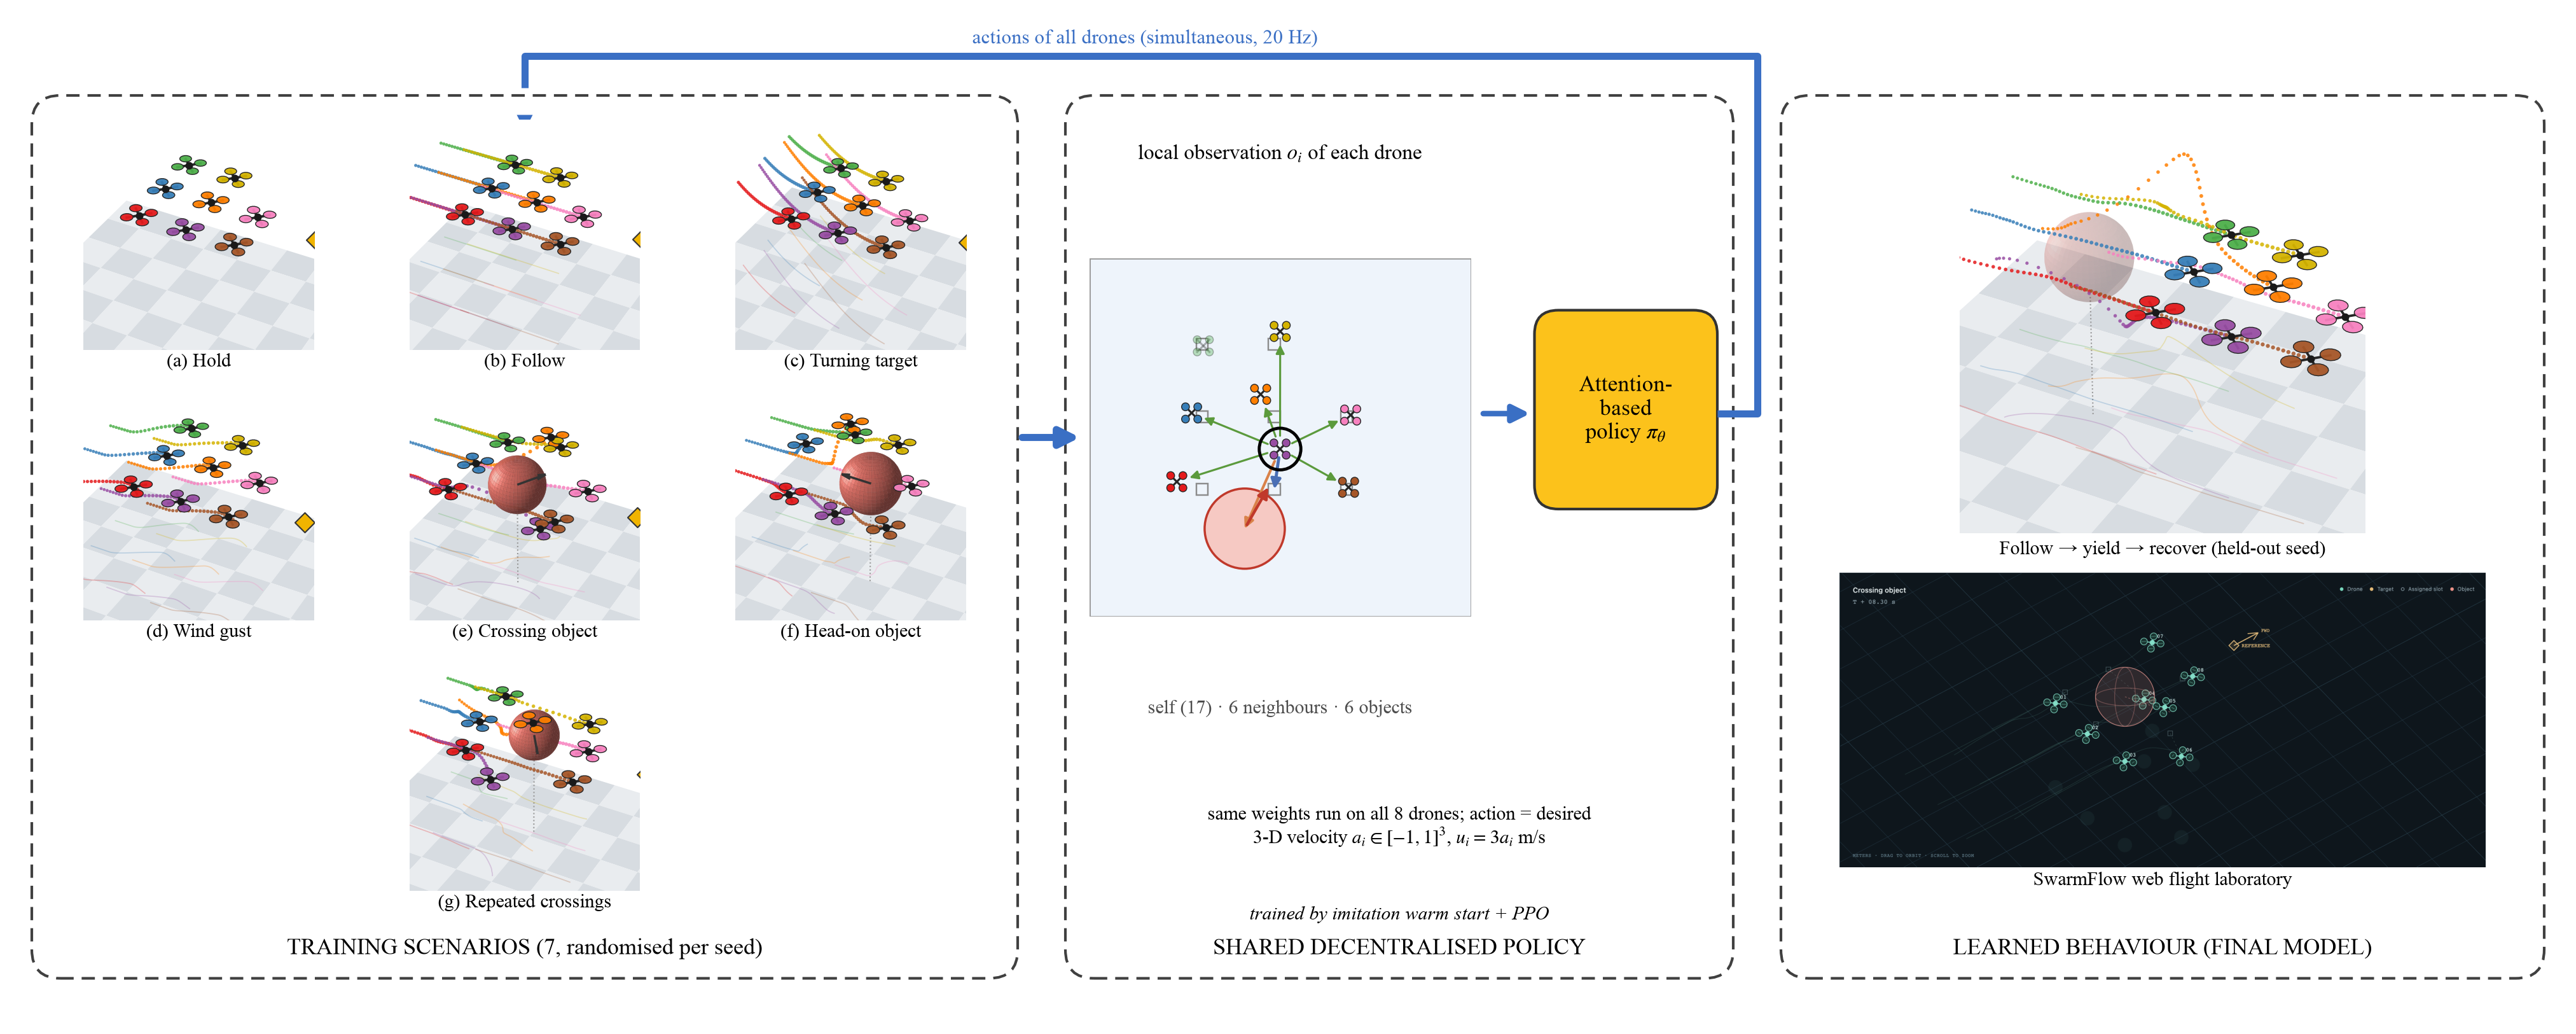
\includegraphics[width=0.84\textwidth]{fig_system_overview}
  \caption[Overview of the proposed reinforcement-learning drone-swarm system]{Overview of the proposed system.
  Left: the seven training scenarios, rendered from the simulator. Middle: every drone builds a local
  observation and the shared attention-based policy maps it to a velocity command; the actions of all drones
  are applied simultaneously. Right: behaviour of the final model on a held-out seed and the web-based flight
  laboratory.}
  \label{fig:overview}
\end{figure}

\section{Need for the Study}
Formation flight with obstacle avoidance involves several requirements that conflict with each other. A drone
that stays exactly in its slot may collide with an approaching object; a drone that avoids the object must
not collide with its neighbours; and after the disturbance the formation must be restored, with every drone
returning to its own place rather than to any free position. Encoding all of these interactions by hand
becomes difficult as the number of drones and the variety of disturbances increase.

A learned, decentralised controller is attractive because the same policy runs on every drone, it uses only
locally available information, and it can in principle be applied to different swarm sizes. However, training
such a controller from scratch is sample-inefficient: published quadrotor-swarm results use very large
training budgets \cite{batra2021decentralized}. A practical project therefore needs a formulation that learns
swarm coordination efficiently on ordinary computing hardware while remaining measurable and reproducible.

\section{Problem Statement}
\label{sec:problem}
The problem considered in this work is to learn a single decentralised policy $\pi_\theta$ for a swarm of
$N=8$ drones such that:
\begin{enumerate}
  \item every drone follows its own persistent formation slot, defined 3\,m behind a reference target that
        moves along a prescribed path;
  \item when a spherical object crosses the formation (laterally, head-on, or repeatedly), the drones avoid
        the object and each other without any collision;
  \item after the object leaves, every drone returns to \emph{its own} slot relative to the moving target;
  \item each drone uses only local, relative observations and the policy weights are shared by all drones.
\end{enumerate}
The behaviour is evaluated on scenarios with unseen random seeds using three measurable criteria: absence of
collisions, formation recovery within 5\,s, and a slot root-mean-square error (RMSE) below 0.35\,m when the
formation is undisturbed.

\section{Objectives}
\begin{enumerate}
  \item To build a multi-agent simulation environment for formation following, obstacle yielding and formation
        recovery with continuous collision detection.
  \item To formulate the task as a decentralised multi-agent RL problem with local observations, continuous
        velocity actions and a bounded reward.
  \item To design a permutation-invariant, attention-based policy network shared by all drones.
  \item To train the policy with a curriculum that combines demonstration-guided initialisation and PPO.
  \item To evaluate the final model on held-out seeds and to demonstrate it in an interactive web viewer.
\end{enumerate}

\section{Scope of the Work}
The drones are simulated with a stabilised velocity-level flight model: the policy commands a desired velocity
and a lower-level controller with finite response time and bounded acceleration tracks it. The learning
therefore concentrates on swarm coordination rather than on rotor-level stabilisation, an approach motivated by
the separation of control levels in \cite{panerati2021learning}. Obstacles are modelled as spheres, sensing is
ideal by default, and the reference target follows a scripted path. Full rotor dynamics and hardware flight
are outside the present scope and are discussed as future work in Chapter~\ref{ch:results}.
